% standard
\documentclass[a4paper,11pt]{article}
\usepackage[utf8]{inputenc}
\usepackage[ngerman]{babel}

\usepackage{titlesec}

\setcounter{secnumdepth}{5}
\setcounter{tocdepth}{5}

\titleformat{\paragraph}
{\normalfont\normalsize\bfseries}{\theparagraph}{1em}{}
\titlespacing*{\paragraph}
{0pt}{3.25ex plus 1ex minus .2ex}{1.5ex plus .2ex}

% geometry
\usepackage{geometry}
\geometry{ headsep=20pt,
headheight=20pt,
left=21mm,
top=15mm,
right=21mm,
bottom=15mm,
footskip=20pt,
includeheadfoot}

% for using wrapfigures
\usepackage{wrapfig}

% header and footer
\usepackage{datetime}
\newdateformat{dmy}{%
\THEDAY.~\monthname[\THEMONTH] \THEYEAR}
\usepackage{fancyhdr}
\pagestyle{fancy}
\lhead{Noah Vogt \& Simon Hammer}
\chead{}
%\rhead{\dmy\today}
\lfoot{}
\cfoot{Gymnasium Kirschgarten}
\rfoot{Seite \thepage}
\renewcommand{\footrulewidth}{.4pt}

% fix figure positioning
\usepackage{float}

% larger inner table margin
\renewcommand{\arraystretch}{1.4}

% no paragraph indent
\setlength{\parindent}{0em}

% graphics package
\usepackage{graphicx}

\usepackage{multicol}

% use sans serif font
\usepackage{tgheros}
\usepackage{mathptmx}

% don't even ask what this is for, I have no idea (noah)
\usepackage{bm} %italic \bm{\mathit{•}}
\usepackage[hang]{footmisc}
\usepackage{siunitx}
\usepackage[font={small,it}]{caption}
\sisetup{locale = DE, per-mode = fraction, separate-uncertainty,   exponent-to-prefix, prefixes-as-symbols = false, scientific-notation=false
}
\newcommand{\ns}[4]{(\num[scientific-notation=false]{#1}\pm\num[scientific-notation=false]{#2})\cdot\num[]{e#3}\si{#4}}

% show isbn in bibliography
\usepackage{natbib}

\begin{document}

\begin{titlepage}

\vspace*{1cm}
	\centering
	
	{\huge\bfseries Eine Email-Client-App entwickeln \par}
	\vspace{0.5cm}
	{\Large Noah Vogt \& Simon Hammer\par}
	\vspace{17cm}

	{\large Geschrieben im Jahr 2021\par}
	
\end{titlepage}

\tableofcontents
\pagebreak

\section{Vorwort}

Ich (Simon) habe lange Zeit mich darüber aufgeregt, dass es keine Edubs-Mail-App gibt. Ich musste die Browserversion als Link auf meinem Smartphone Bildschirm 
einfügen und ich habe mich sehr darüber genervt, dass ich mich jedes mal beim öffnen der Browserversion neu anmelden musste. Als dann die Zeit kam mich für eine 
Maturarbeit zu entscheiden, wollte ich zuerst einen Edubs-Client erstellen, welcher für Schüler gut geeignet ist. 
Jedoch kannte ich bis dort nur Python und wollte mich mit meiner Idee mit Noah unterhalten, 
da ich wusste, dass er sicher auch etwas programmieren wird, weil er sich schon seit längerem mit Computern und der Programmiersprachen befasste. Er war der Meinung, ich könnte dies
doch gleich für jede Art von Email machen. Da ich mich noch nicht gut mit dem Programmieren auskannte, fragte ich ihn, ob er diese Maturarbeit denn mit mir machen würde.
Zu meiner Überraschung war er von der Idee überzeugt und wir einigten uns darauf, einen Email-Client zu erstellen, welcher zwar nicht für Schüler optimiert wurde, aber für 
den allgemeinen Gebrauch verbessert wurde. 

\section{Einleitung}
Das Kommunikationsmittel Email ist auch nach seinem fünfzigjährigen Jubiläum noch rege im Alltagsgebrauch vieler Leute in den meisten (industrialisierten) Ländern. Es könnte angenommen werden,
dass sich auch in den letzten zehn Jahren - nämlich seit dem Aufkommen der massentauglichen Smartphones - die Emailsoftware verbessert hat. Doch für das Smartphone war es für uns, die Ersteller dieser Maturarbeit, schwer einen guten Email Client zu finden. Diese Maturarbeit ist unser Teil, daran etwas zu ändern, wenigstens für uns.


\subsection{Ziel der Arbeit}

 was, wie und warum [machen wir das?]

\section{Konzept der Arbeit}

\subsection{Ziele der Funktionen}

Wir kennen alle die Funktionen eines Email-Clients und unsere App soll auch nicht viel mehr können als die meistens Apps. \\

Die App soll die Basisfunktionen eines klassischen Email-Clients erfüllen. Dazu gehören das lesen und schreiben von Emails,
öffnen und Anfügen von Anlagen, die Setzung einer Email-Signatur und das Erstellen und Speichern von Entwürfen. Ebenso soll es viele verschiedene Ordner geben, 
solche wie Spam/Junk oder ein Archiv Ordner. Dazu soll es möglich sein E-Mails verwalten zu können, zum beispiel indem die Ordner nach 
Datum des Empfangs oder dem Absender sortiert werden können. E-Mails könne markiert, gelöscht und weitergeleitet werden. Es soll eine Suchfunktion für jeden Ordner geben. \\

Ebenso soll es einen Account Manager geben, was voraus setzt, dass es möglich ist sich mit verschiedenen 
Accounts anzumelden und diese bei bedarf zu wechseln. Beim Anmelden einer E-Mail soll es dem Nutzer leicht gemacht werden mit eingebauten Konfigurationen für beliebte 
Emailprovider in der Schweiz. Darunter diese Anbieter: stud.edubs.ch, gmail.com, gmx.ch, outlook.com, yahoo.com, icloud.com, hotmail.com, web.de. \\

Ein Element, welches fast jede App Heutzutage hat, sind Pushnachrichten, welche auch eingebaut werden sollen. Dabei wird die Nachricht mit dem Absender und der Beginn der 
E-Mail angezeigt. 
Eine Funktion die nicht jeder Email-Client hat ist, dass die Gesprächsverläufe in der Struktur wie auf Reddit oder Thunderbird gezeigt werden. 
Dies wird ein weiteres Feature der App sein.
Wie es für leichte Email-Clients oft üblich ist, werden Bilder erst angezeigt, sobald es der Nutzer ausdrücklich möchte. Für dies 
wird eine Funktion in den Einstellungen  einfügen. Eine sehr praktische Funktion soll sein, dass E-Mail-Adressen gespeichert werden und 
beim schreiben einer neuen E-Mail direkt verfügbar sind und ausgewählt werden können. \\

Das letzte Feature ist, dass Links direkt in einem Browser geöffnet werden können. Die Einstellungen sollen das Farblayout der App ändern können, 
die Synchronisationsintervalle ändern können, Einstellungen an den Pushnachrichten ändern können, Kontaktlisten verwalten und Einstellungen zu Privatsphäre beinhalten. 

Ein Pluginmanager soll auch eingebaut werden, um weitere Funktionen, welche das Programm verlangsamen würden oder nicht für jedermann geeignet ist, hinzuzufügen können. 
Es gibt uns auch die Möglichkeit nach dieser Arbeit die App zu verbessern und auf uns an zu passen. \\ 

Wir haben uns viele Ziele gesetzt und dachten, dass wir auch mehr schaffen können. Weshalb dies nicht der Fall ist wird noch genauer betrachtet. 



\subsection{Vergleich mit Konkurrenz}
Disclamier/Note: Da bei dieser App einen Wert auf Sicherheit und Endnutzer-Freiheit gesetzt wird, wird sie dementsprechend nur mit Apps verglichen, welche auch Freie Software sind, nach Definition [der FSF??]. Somit fallen jegliche Proprietäre Produkte raus, da sie unseren Grundanforderungen eines Email Clients nicht entsprechen.\\


Wenn wir die meisten anderen quelloffenen, noch maintainten Open Source Email Clients anschauen fällt sofort auf, 
dass diese unglaublich überladen (bloated) sind. Selbst wenn im Internet nach einem möglichst simplen Email Client für Android gesucht wird, 
stösst man dabei meist auf Apps wie k-9 Mail, welche hunderttausende Zeilen Source Code besitzen.\\

Im Unterschied zur Konkurrenz soll diese App so programmiert werden, dass sie alle nötigen Grundfunktionen für einen Email Client auf dem Smartphone beinhaltet, 
aber schneller starten soll als die Apps der Konkurrenz, weniger Speicherplatz und Resourcen verbrauchen soll und nicht mit unnötigen Funktionen überladen sein.

\subsection{Quellcode Modell}
Um ein Programm zu programmieren, werden menschenlesbare Instruktionen in ein oder mehrere Textdateien geschrieben,
die dann in Sprache, welche die Computerhardware interpretieren und ausführen kann, übersetzt. 
Bei diesem Prozess geht die Lesbarkeit für den Menschen grösstenteils verloren. Um ein Programm ausführen können braucht der Nutzer also keinen Zugang zum Quellcode. Doch wenn er wissen will, was das Programm macht - es könnte ihn ausspionieren oder andere bösartige Sachen im Hintergrund machen - oder einfach das Programm verändern will, braucht er unbedingt Zugang zum Source Code.\\

Durch die zunehmende Kommerzialisierung und Massentauglichkeit der Computer haben sich aber monetäre und andere Anreize gebildet, den Source Code dem Nutzer nicht mehr zur Verfügung zu stellen. Das hat für den Nutzer verschiedene praktische Folgen. Aber vor allem ist er nicht mehr in Kontrolle seines Computers, Betriebssystems und Programms, sondern der Besitzer oder Copyrightholder des Programms. Das ein Programm einen Besitzer haben kann, ist ziemlich absurd und nur durch die Veränderungen der westlichen Copyright- Gesetze- und Kultur der letzten 150 Jahre [möglich?].\\

Doch auch bei Open Source Software gibt es verschiedene Lizenzmodelle welche gewählt werden können. Diese lassen sich gut ein zwei Kategorien unterteilen:\\

\textbf{Permissive Licenses:}
These give you the right to run the program for ANY purpose, study the source code, change it and redistribute the changes. Their names come from the fact, that they are ``permissive'' when it comes to their few restrictions: They do not put of a lot of restrictions on the distribution of the source code, and often allow the software to be forked under ANY terms. This means it is possible to make your fork of a permissive-licensed program proprietary.\\

This means they do not protect their code from being taken and used in other projects, even proprietary, without any giving back, which is a definite drawback and the reason people insult these licenses as ``cuck licenses'' as you ``write proprietary code for free for big tech without increasing anyone's computer usage freedom''. A positive point of these licenses however is their simplicity: The MIT license for example only consists of 20 SLOC, while a Copyleft license as the GPL v3 uses more than 600 SLOC and its jurisdictional jargon is much harder to understand.\\

\textbf{Copyleft Licenses:}
This is an obvious play on the word ``Copyright'', as it tries to invert its effects. As with permissive licenses you can run the program for ANY purpose, study, change the source code and redistribute the changes. But the trick comes with their restrictive redistribution terms: You can ONLY redistribute the program if your version provides the same user freedoms. This is usually done in only allowing redistributing using the same license.\\

To provide such protection of the user freedoms in future forks, there needs to be a lot of jurisdictional jargon in the license which makes it significantly longer and harder to understand for the average reader. But most of the people in Free Software who care about user freedom say this is the premiere license for your free software projects, as it ensures that freedoms have to be granted forever and stopping proprietary code maker profiting from their written free code.\\

\subsection{Philosophie (suckless)}
(Nowadays) a lot of Open Source Developers pride themselves in writing software with much features that cater to the non-technical enduser. This results in having a large codebase, which gets bigger and bigger with every release. This makes it harder to maintaining the ever growing codebase, more and more bugs occurs, security and (most importantly) performance struggles under these conditions. This degrades the quality of software technology as it is the mainstream narrative to ``save time and money''.\\

This is where the ``suckless philosophy'' comes in place: It aims at making software with simplicity in mind: Less source lines of code to not render the project unmaintainable in similar way as mentioned above. This way of programming is a lot more difficult, but the struggle is most of the time worth it. This coding philosophy also incentives (quality) code rewrites - which happens a lot less with bloated software counterparts - that gives the user more alternatives to choose from.

\subsubsection{Hintergründe, Technologisch, UNIX, KISS}
\subsection{Lizensierung}
%The differences of different source code models and their licenses have been already discussed in this paper (?). The reason the GNU General Public License Version 3 (short: GPL v3) was chosen because it is one of the most popular and strongest copyleft licenses that suits the application.

Die Unterschiede zwischen verschiedenen Source-Code Modellen und deren lizenzirrung wurden bereits besprochen. Der Grund weshalb die GNU General Public License Version 3 (kurz: GPL v3) ausgewählt 
wurde, ist dass sie eine der bekanntesten und stärksten copyleft Lizenz ist.


\subsubsection{Hintergründe, philosophisch, technologisch}

\section{Hilfsmittel}

\subsection{Hardware}

\subsubsection{Smartphones}
%We used different Models of Smartphones running different variants of the android operating system to install and test our app. It was also used to compare it and benchmark it against our competition (the already existing mail clients on android).

Es wurden verschiedene Smartphone Modelle genutzt um die App auf verschiedenen Androidversionen testen zu können. Sie wurden auch genutzt um unsere App mit der Konkurrenz zu vergleichen und die 
Konkurrenz zu begutachten. 

\subsubsection{PC / Laptop}
%The usage of computers was to the actual work of creating the software, documentation and the text of this paper (?).

Der Gebrauch von Computern wurden gemacht um die Software, die Dokumentation und dieses Maturschreiben zu erstellen. 
\subsection{Software}

Aufgrund dessen, dass ein umfassendes Programm entstehen soll, wird auch Gebrauch von einigen anderen Programmen, Bibliotheken und sonstigen Tools gemacht. In den nachfolgenden Seiten wird beschrieben welche Programme genutzt werden, wieso diese ausgewählt wurden und wie der Umgang mit Ihnen war.  


\subsubsection{Programme}

\paragraph{Version Control System}

For developing software above a certain level of complexity, it helps to use a so called VCS (Version Control System). This is a software/system that manages the versioning of software. This is useful so you don't have to for example create MANUALLY a new folder for every new version and copy the code with the new changes in there. This would be not very user friendly, wasteful of disk space and overall very inefficient. These systems also make it easy to synchronise projects to a remote server to allow for easy collaboration on multiple devices and for different developers.\\

It also allow for additional advanced features like branching a repository, which means developing multiple features separately from each other to then later merge the changes together, when each of the features are working as expected.

\subparagraph{Git}

Git und GitHub sind wohl die wichtigsten Programme die genutzt wurden. Sie sind Systeme, welche Fileordner (repository) verwalten können und sie für mehrere Computer zur Verfügung stellen, 
wobei sie sehr viele praktische Funktionen mit sich bringen. Mit Git können repositories local auf Computer oder Hardware geteilt werden, mit GitHub könne die repositories auch 
über das Internet geteilt werden. Der einfachheitshalber wird nicht zwischen Git und GitHub unterschieden. 

\subparagraph{Github}

This is our remote git server. But is is more than just a git server, it is a popular platform with over 50 million (software) repositories that people search to find interesting software. So we can use this to make our software more searched and popular (but this is not considered of great importance).

\paragraph{IDE}
IDE stands for ``Integrated Development Environment''. This means a program where the coder edits, debugs the code. It provides more features than just editing text, but also advanced autocompletion features and warnings/suggestions that the programmer should do something differently because of various reasons of bad programming practice. These programs have a lot of great features, but are often buggy, resource hungry and slow, like our choice of IDE: Android Studio.

\paragraph{Texteditor}
Text editors to have less ``advanced'' coding-related features, so they are not optimal for big projects with lots of files and graphical content.

\paragraph{Android Emulator(s)}
An emulator is a program that simulates an device/operating system so that you can run inside another operation system. We use an Android Emulator inside of our GNU/Linux running on our computer, so that we do can test our app without always having to transfer it to an actual phone running android natively.

\paragraph{Compiler}
gradle, maven

\paragraph{Installer / Packaging}
When we compiled our app using gradle, we get an .apk file as its output. APK stands for Android Package, which is the Package Format used for installing most of the software in Android. However, there are to sorts of apk that are compiled: a debug apk and a release apk. The debug version has extra features compiled in that help auditing bugs and new features not ready for using in the app available to users. The release Version has the current version number (?) added to it and is what you need to distribute of your working version to your users.

\subparagraph{signing keys}
Nearly all Android Systems are configured to only allow application that are signed with a key from the developers. This is done for various reasons like security, compatibility checks and other (TODO: search more on this). So before we can install our app on 99\% of Smartphones, we first have to sign it with our cryptographic key we have created. Of course, this is only needed for actual releases and not for using debugging version e.g. in your android emulator.
\subparagraph{Android Debugging Bridge}
This is a software tool to interact with android devices that are connected to a computer via usb. With it you can do useful thinks like screenshots, screen recordings, transferring files to and from your computer and installing / removing packages.

\paragraph{Open Source Programme}

Beim Programmieren kann es sehr Hilfreich sein Programme zu haben welche, ähnliche Funktionen haben wie das Programm welches entstehen soll. 
Solche Vorlagen können beliebig getestet und verändert werden. Simon hatte zu beginn Schwierigkeiten Java zu nutzen, um Programme zu schreiben, da er noch nicht viel 
Erfahrung mit dem Programmieren hatte. Um sich mit der Art der Sprache und des Programmierens vertieft auseinander zu setzen, begann er Email-Apps, welche Open Source
waren, genauer zu Betrachten. Im folgenden Text werden wir diese Programme aufführen und zeigen für was wir sie gebraucht haben. 

\subsubsection{Librarys}
(bedeutung im glossar erklärt)

\paragraph{RecyclerViewer}

Der Recyclerviewer ist ein Behälter in welchen Daten gepackt werden. Er wird dem Layout hinzugefügt und hat eine grossen Vorteil gegenüber Listen. 
Eine Liste wird einmalig erstellt und komplett generiert. Das heisst es gibt Behälter, welche existieren, aber nicht auf dem Bildschirm angezeigt werden. 
Diese Behälter brauchen aber dennoch Speicherplatz, sind aber sinnlos. Hingegen der Recyclerviewer generiert nur so viele Behälter wie auf dem Bildschirm angezeigt werden können. 
Die Behälter, welche beim Scrollen am Bildschirm ende ankommen werden sogar wieder verwendet, mit neuen Information gespeist und am anderen Ende des Bildschirms angezeigt.

Bild von RecycleView

Ich (Simon) habe viel Zeit in einem template für den Recyclerviewer verbracht, da mir viele Internetseiten nicht helfen konnten. Es waren die ersten Schritte um 
richtig zu verstehen wie eine App funktioniert und wie sie Aufgebaut ist. Ich habe mich davor schon informiert jedoch wurde es mir dort richtig klar. Ich habe gelernt
wie Behälter über einen Key von Java Files aufgerufen werden und mit Daten gespeist werden. Ebenso habe ich verstanden, weshalb in Programmen, basierend auf Java, viele 
Klassen erstellt erstellt werden müssen, weil jeweils nur einmal die Variablen, Funktionen und Konstruktor einer andere Klasse implementiert werden können. Das heisst, 
wenn eine Klasse zwei Funktionen aus zwei unterschiedlichen Klassen verwendet werden soll, muss eine der beiden Klassen die andere Klasse implementieren. 

\subsection{Recherche Tools / Quellen}
\subsubsection{Internet}
In the world wide web we use search engines like DDG (duckduckgo.com), the Arch Linux Wiki, Wikipedia and more programming-related websites like SOV (stackoverlow.com).
\subsubsection{Bücher, Artikel}
We used different books and articles physically and digitally sometimes for the programming/coding process, but mostly for the text of this paper.

\subsection{Dokumentation(-stools)}
\subsubsection{Latex}
To write more formatting-demanding papers like in this paper it was made use of the typesetting engine LaTeX. This is a highly extensible and efficient way for getting your paper to look just like you want it. Also professionals use it to format a big majority of published books since \~ 20 years up to this day(TODO: look up on facts/statistics for this).
\subsubsection{Pandoc}
This is program to convert from one document format to another. This is useful to write a document in format with very simple syntax (e.g. markdown) to convert it to a format that allows much better formatting (e.g. LaTeX) without having to use the more sophisticated syntax of the latter format. This is often used to write documentation or short texts with the minimal amount of time and effort to do so.

\section{Programmstruktur}

\subsection{Sicherheit / Security (Features)}
    Considering that on 99\% of consumer smartphones the users do not even have root access (but which the ``owner'' of the smartphone software do have), people that are concerned with privacy or security would not use their important mailboxes on their smartphone anyway, but rather on their better secured computer running a Free Software Operating System etc.\\

Also taking in mind that the email protocol was written in a time with a still very limited access to computers, privacy and security where not in mind of its creators at the time is quite understandable. Why it still lasted to this day in this state is compromised on one side by networking effects and on the other side that simply most people neither know to technical detail nor care.\\

Nowadays it is possible to encrypt to content (body) of an email, but not the metadata, here the specification of the email protocol is to blame. This and just the fact that is was not BUILT as a secure or private way of messaging, makes emails not useful for these kinds of conversation. If you want to send your friends new plans on overtaking the world and establishing a global catholic monarchy without wanting anyone to know, your are a fool if you use email for that(granted, this is an over exaggerated example, but I hope the idea is clear).\\

So the conclusion for our application project is to not bloat up our app with hard-to-use security functions that just bloat the app and codebase unnecessarily. However we use sane security-focused default now further explained.
\subsubsection{PRIVATE MODE, Sandbox}
When storing user settings (and data?), you can choose between different permission modes in android. We choose PRIVATE MODE, which means that apps with user permissions  can not see its content. But Google, root users, and apps with root access can easily bypass this restriction of the android permission system.\\

To prevent this type of exploitation we would have to encrypt ALL sensitive user data with an encryption key. But when there is a keylogger installed, even this is not safe. So considering that there is not a single android phone free from proprietary operating system and firmware code(when connecting to the internet via WiFi), this feature idea has been rejected as out of place and to make our codebase simpler.

\subsection{Code Kompaktheit}
This is something that we have absolutely achieved, we used so much less SLOC than any of the competing email clients on android.(TODO: compare use of libraries, and if we used more or less than the other apps) This is also very crucial to stand with our initial goal and the suckless philosophy. While we used \~ 4000 SLOC, other apps use a whopping 300'000 SLOC.
\subsubsection{Maintaining}
Our codebase should be very easy to maintain: The main things you would have to do is check if the dependencies are up to date and if they can be considered deprecated.\\

Even if this project gets abandoned by their original developers - or as some people call that: when it get orphaned - and if someone finds it and likes it, he can easily read through it and understand the code without too much effort needed of understanding the codebase. Would the same be the case for bloated programs like thunderbird? I don't think so either.
\subsubsection{less bug/error-prone}
This is thanks to the suckless nature of our coding philosophy, but also our execution. It could be the case however that bad practices may have been used as the initial project owner did not have a lot of experience of java or android coding.

\section{Umsetzung}

\subsection{Informationsbeschaffung}

Zu beginn der Arbeit konnten Noah und Simon noch kein Java. Noah kannte sich gut aus mit Programmiersprachen und konnte es deshalb mit Java ruhig angehen.
Simon hingegen wusste, dass er noch viel zu lernen hatte. Er erhoffte sich die Grundlagen im Informatik Unterricht zu lernen. 
Simon lernte auch einige dinge, jedoch ging ihm das zu langsam und er schaute sich nach anderen Lernmöglichkeiten um. 
Zu diesem Zeitpunkt konnten einige Schüler an einem Programm mitmachen, bei welchem sie in die Uni gingen und gewisse 
Vorlesungen besuchen konnten. Ein Klassenkamerad von Simon konnte von diesem Programm profitieren und besuchte Informatik. 
Dort lernte er in einem unglaublichen Tempo Java, weshalb Simon seinen Klassenkameraden fragte ob er seine Unterlagen ausleihen konnte. 
Sein Klassenkamerad war so freundlich und übermittelte ihm die Unterlagen. So konnte Simon auf effektive weise Java lernen. \\

\textbf{ Noah wie hesch du Java glernt?}<++>

Als nächstes ging es darum wie eine App aufgebaut ist und wie zwei Personen Zweitgleich an einem 
Programm arbeiten konnten. Dafür musste sich Simon über Git/Github informieren. Noah hatte ihm ein Video empfohlen, welches 
Simon studieren soll und er soll kleine Übungen mit Git ausprobieren um ein Gefühl dafür zu bekommen. Die beiden Informierten 
sich über verschiedene Plattformen wie eine App funktioniert und wie sie aufgebaut ist. \\ 

Es ging langsam voran und die beiden begannen mit technischen Einstellungen. Als erstes 
wurde Android Studio  und eine ADB installiert. Noah hat sogar eine Anleitung zur Installation von ADB geschrieben. 
Um diese auszuprobieren und die Grundlage zu schaffen auf welcher Simon und Noah die nächsten paar Monaten arbeiten werden, haben sie ein
Testprogramm erstellt namens "Hello World". Es war ein ganz simples Programm das nur zum Testen der Infrastruktur diente. 
Sie haben ein Gradle.build file erstellt, dies dauerte erstaunlich lange. Später erkannten sie das diese Verhalten sehr üblich für 
Gradle ist. Nach einiger Zeit haben es beide geschafft ein apk file zu besitzen, welches erfolgreich die "Hello World" app beinhaltete und ausführt. 
Anschliessend erstellte Noah ein GitHub repository in welchem die beiden das Programm teilen werden. \\

\textbf{ https://www.youtube.com/watch?v=2sjqTHE0zok} nur um später zu makieren.

\subsection{Interface}

Noah begann dann dieses Programm leicht auszubauen und fügte einige Interface Inhalte hinzu. 

\begingroup
\setlength{\intextsep}{10pt}
\setlength{\columnsep}{15pt}

\begin{wrapfigure}{r}{8cm}
\centering
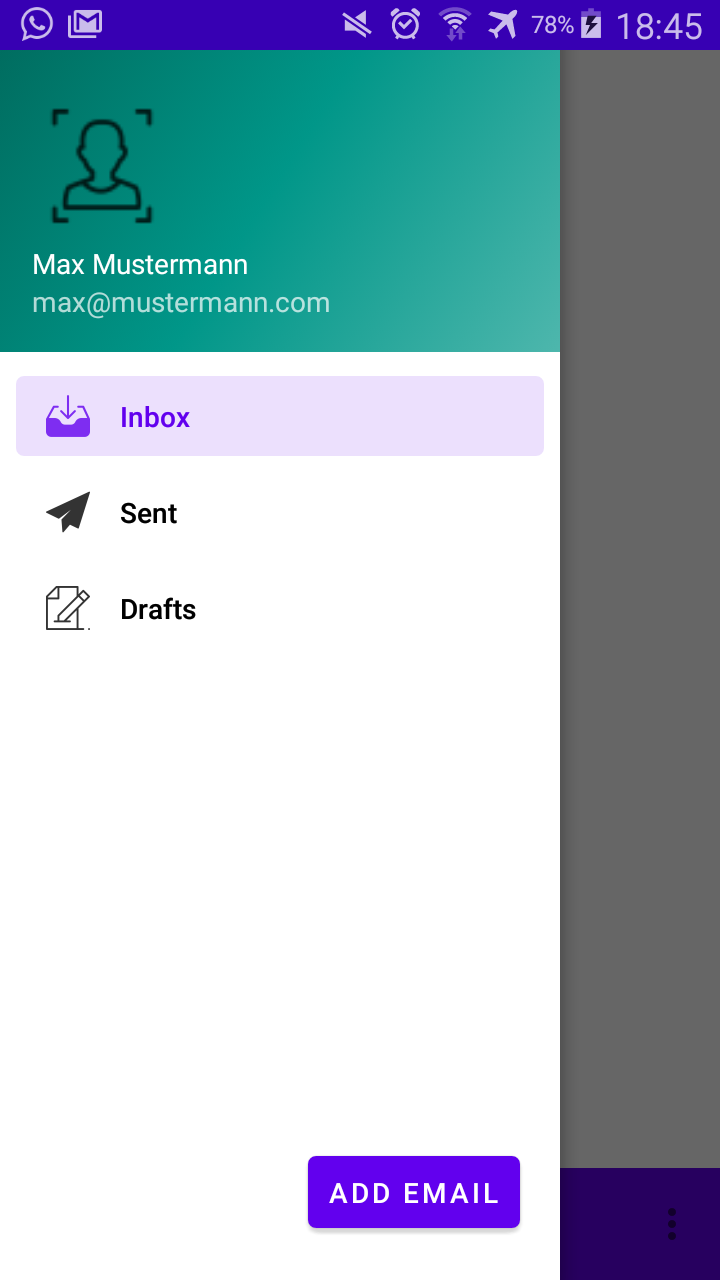
\includegraphics[scale=.15]{media/drawer.png}
\caption{Drawer Navigation Menu}
\end{wrapfigure}
%I then made the app more functional, so that you have a base GUI with a drawer, a menu in the bottom and in the drawer navigation menu you can tap on the «Add Email» Button and a popup window will come up asking you for name, email and password. Even the save and cancel button work. Now we only need a functionality to save this information to a string somewhere in the main activity.\\

Die App beinhaltete ein Burgermenü mit drei Ordnern und einem Knopf, welcher den Nutzer zu einem Popupwindow führte, in welchem es so aussah als würde es möglich sein sich anzumelden.  
Die Basis für die App wurde gelegt und die beiden entschieden sich mit dem Interface anzufangen. Für Simon ein guter Anfang sich mit dem 
richtigen Programmieren zu befassen und sich einleben zu können. 
Simon begann mit dem RecyclerViewer



\subsection{Beispiele aus der Umsetzung}
\subsubsection{Bugs}
Erklärung woher, warum falsch, wie gelöst
GUI stuff -> onliner commit 

\subsubsection{Probleme / Hiccups}
RecyclerViewer, shit java IMAP libraries

\subsubsection{Kommunikation}
simon fragen, war Kommunikation zwischen uns gut?

\section{Einschätzung / Schlussfolgerung}

\subsection{Fremdeinschätzung}
\subsection{Selbsteinschätzung}
\subsubsection{was lief gut}
komm., vcs, java syntax (allg.)
\subsubsection{was lief schlecht}
******* java shit tier libraries
\subsubsection{was würden wir gleich machen}
As long as java is not deprecated in the future for android programming, we would still use it as it is the most ``native'' way of programming. The new java clone/fork of google, Kotlin, would be a worse choice in our eyes, as your are even more dependent on google code, which you are already by using android.
\subsubsection{was würden wir anders machen}
As java is much slower than language that can be compiled into native binaries we would try to use more C or C++ libraries to improve speed and portability. 


use more c libs for speed and less java (that's always a good thing)
\subsubsection{abschliessende persönliche Schlussfolgerung}

\section{Danksagung}


\end{document}
